\subsubsection{Cliente}

En esta sección se describirá la implementación del cliente del juego, detallando su estructura, componentes 
y cómo se integra con el resto del sistema. Se explicará la organización del proyecto en \texttt{Unity}, la 
arquitectura de sus módulos, la comunicación con el servidor y las herramientas utilizadas para su desarrollo.

El cliente contiene tres módulos principales: el \texttt{Core}, que contiene la lógica central y utilidades; 
el \texttt{Gameplay}, que maneja la lógica de juego en tiempo de ejecución; y el \texttt{User Interface}, 
que se encarga de la representación visual y la interacción del usuario. Para más detalle sobre \texttt{módulos}, 
\textit{Assemblies} y \texttt{Vcontainer}, esto se explica en la sección de 'Estructura del proyecto de Unity'.

% TODO: (reference) 8.2 Estructura del Proyecto de Unity

\paragraph{Core}

Un elemento primordial en la capa de \texttt{Core} del cliente es la implementación del sistema de inputs del cliente, 
el cual se basa en el sistema de inputs de \texttt{Unity}, pero con una capa de abstracción que permite una mayor 
flexibilidad y modularidad. Este sistema de inputs se integra con el resto del cliente a través de eventos, 
lo que permite que cualquier componente pueda reaccionar a las acciones del usuario sin necesidad de conocer 
la fuente de esos inputs.

Se encuentran en el \texttt{Core} también varios gestores de recursos, como el gestor de Menú, de controlador del 
\textit{mouse}, de la cámara y otros, que se encargan de manejar aspectos específicos del juego y proporcionar una 
interfaz para interactuar con ellos.

\vspace{0.20cm}

Dentro del módulo de \texttt{Core}, también hay un \textit{assembly} llamado \texttt{Common}, donde se guarda 
la lógica y los datos que deben ser idénticos para cliente y servidor. 

Dicho módulo, no contiene código de \texttt{UI} ni de \texttt{Gameplay} exclusivo, sino contratos, 
configuraciones y mecanismos de red que ambos lados usan para comunicarse. 
Esto garantiza que interpreten igual los valores de configuración y protocolos. 
Entre estos se encuentran \textit{DTO's}, \textit{Enums}, eventos, y otros elementos compartidos. 

\paragraph{Gameplay}

El módulo \texttt{Gameplay} es la capa de jugabilidad y ejecución específica del cliente. No es solo lógica de red ni 
solo \textit{UI}, es el conjunto que une la experiencia del jugador con los datos de mundo, con el servidor y 
con los objetos lógicos y visuales que se representan lo que el usuario percibe.

El flujo comienza en sus puntos de entrada (\textit{Entry Points}), donde se maneja el arranque 
del cliente y toda la configuración necesaria para que la escena tome los recursos necesarios para funcionar. 

En el cliente se manejan distintas escenas para cada parte del juego, 
una escena para el menú principal, que incluye el navegador de mundos, edición de personaje y menú de obtención 
de moneda de juego, y otra escena a la que se redirecciona una vez seleccionado un mundo, donde se desarrolla la 
experiencia de juego.

\begin{figure}[H]
\centering
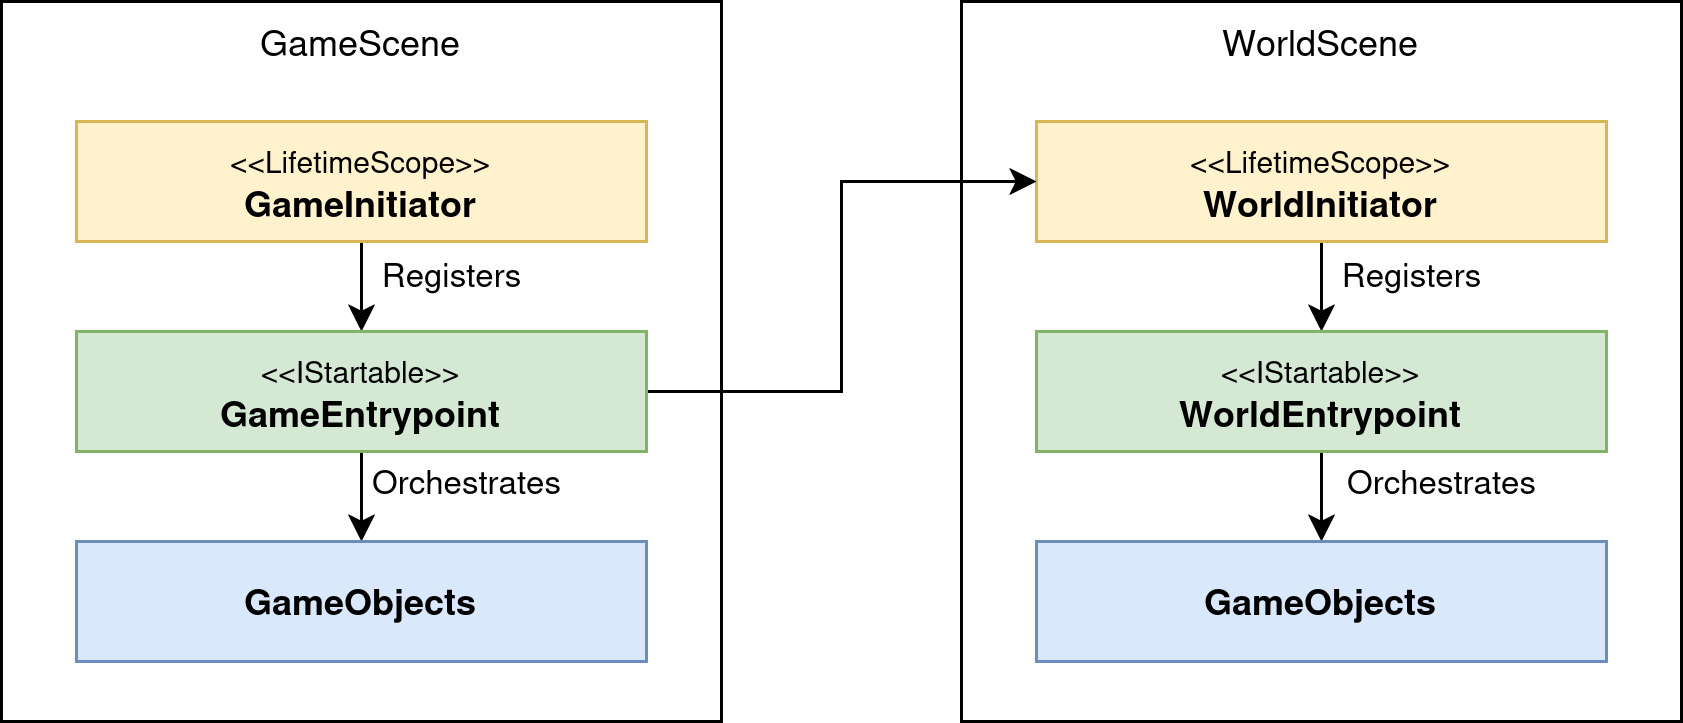
\includegraphics[width=1\textwidth]{img/08-implemented-solution/game/client-init.jpg}
\caption{Visión general del flujo de inicialización del cliente.}
\end{figure}


En cuanto a la configuración de la escena del juego, cada objeto/entidad carga sus datos por su propio sistema 
categorizado de \textit{loaders}. Una vez que se ha establecido la conexión con el servidor y 
se han cargado los recursos necesarios, el \textit{Entry Point} del mundo se encarga de configurar todos los 
objetos presentes en el mismo mediante \textit{linkers}.
Estas son clases que se encargan de vincular al objeto/entidad del mundo con su representación visual y lógica 
en la escena.

Es una capa de \textit{“composition wiring”}: toma objetos de red y los convierte en entidades 
jugables con su \textit{UI} y comportamiento. Esto permite inyectar dependencias y controladores en cada tipo 
de entidad, diferenciar entre jugador local y otros clientes, y dejar las entidades listas para que el sistema 
de juego las maneje sin necesidad de acoplar la lógica de red o de \textit{UI} directamente en ellas, respondiendo 
a lo que el servidor envía y a lo que el jugador hace.

\vspace{0.20cm}

Un componente importante dentro del concepto de \textit{linking}, es el \textit{network adapter}. Este actúa como 
el puente directo entre cada entidad y la red. Para el jugador local, permite que esa entidad envíe acciones y 
transacciones al servidor. Para entidades remotas, permite recibir eventos del servidor y procesarlos localmente.
De esta forma llega información como ataques, diálogos, portales, interacciones, etc. y se procesan en 
cada entidad para que el jugador vea la respuesta a sus acciones o a las acciones de otros jugadores.

Con esto se logra manejar el comportamiento de cada entidad desde la lógica en el servidor, 
y el cliente solo se encarga de representar y ejecutar lo que el servidor le indica.

\paragraph{User Interface}

El módulo de \textit{UI} del cliente es la capa que entrega toda la experiencia visual e interactiva del jugador 
fuera de la simulación de jugabilidad. Su función es presentar información, opciones y controles al 
usuario, y traducir las acciones de la interfaz en eventos que el resto del cliente consume.

Se integra con el resto del cliente mediante eventos y controladores de cada elemento de \textit{UI}. De esta forma, 
al tener la \textit{UI} en su propio módulo, el cliente puede cambiar la presentación sin modificar la lógica de 
\textit{gameplay} o red, por lo que no hay dependencias entre la lógica de juego en el módulo \texttt{Gameplay} 
y la presentación visual.

